\documentclass[aspectratio=169, 11pt]{beamer}
\usepackage{graphicx} % Required for inserting images
\usepackage{tikz}
\usetikzlibrary{shapes, arrows}
\usetikzlibrary{arrows.meta}


% --- Preamble & Fonts ---
% Removed fontspec commands as they often cause issues in limited compilation environments.
% The default beamer fonts should be sufficient for stability.
% If custom fonts are critical, we might need to resort to a different configuration.
\usepackage{amsmath}
\usepackage{algorithm}
\usepackage{algpseudocode}
\usepackage{tikz}


\definecolor{DarkBlueContour}{RGB}{0, 0, 150}
\definecolor{LightBlueFill}{RGB}{173, 216, 230}


% --- TikZ & Beamer Overlay Setup ---
\tikzset{
    alt/.code args={<#1>#2#3}{%
        \alt<#1>{\pgfkeysalso{#2}}{\pgfkeysalso{#3}}%
    },
    highlight/.style args={<#1>}{%
        alt=<#1>{ fill opacity = 0.9,
            draw opacity = 0.6,
            line width=1.5pt
        }{ fill opacity = 0.3, draw opacity = 0.3
        }
    },
    % The style for edges
    edge/.style={
        thick, 
        black!70,
        >=latex,
        opacity=0.3
    },
    vertex/.style = {
        circle,
        draw=DarkBlueContour,
        fill=LightBlueFill,
        minimum size=20pt,
        inner sep=0pt,
        fill opacity=0.3,
        draw opacity = 0.3,
    }
}

\title{Parcours en Largeur — Breadth-First Search}
\subtitle{Illustration de l'Exécution}
\author{Algorithmes et Pensée Computationnelle \newline \newline  {\small UNIL — École des Sciences Criminelles}}
\date{}

\begin{document}

\begin{frame}
\titlepage
\end{frame}


\begin{frame}{Description de l'algorithme}


\begin{enumerate}
\item Initialisez\!:
\begin{itemize}
    \item une \texttt{file} (file FIFO — de type liste) qui contient initialement le sommet de départ.
    \item une liste, appelée \texttt{visited}, de sommets visités qui contient initialement le sommet de départ.
    \item une liste, appelée \texttt{order}, qui stocke l'ordre d'enlèvement de la \texttt{file} — sommets proches au sommet de départ au début de la liste.
\end{itemize}

\item Tant que la \texttt{file} n'est pas vide, répétez les opérations suivantes\!:
\begin{enumerate}
    \item Retirez le premier sommet de la file (utilisez \texttt{pop} en Python ou \texttt{remove} en Java) et appelez-le $u$. 
    \item Ajoutez $u$ à \texttt{order}
    \item Pour chaque sommet adjacent $v$ de $u$\!: si $v$ n'est pas dans \texttt{visited}, alors :
        \begin{itemize}
            \item Insérez $v$ à la fin de la \texttt{file}.
            \item Insérez $v$ à la fin de \texttt{visited}.
        \end{itemize}
\end{enumerate}

\item Retournez \texttt{order}.
\end{enumerate}


\end{frame}

\begin{frame}{Exemple du graphe}
Dans cet exemple, nous prenons un graphe avec la liste d'adjacence:
\[
\left\{
\begin{aligned}
    A &:[B,\, C,\, D,\, E], \\
    B &:[\ ], \\
    C &:[\ ], \\
    D &:[E], \\
    E &:[F], \\
    F &:[\ ]
\end{aligned}
\right\}
\]

\end{frame}

% --- The Frame ---
\begin{frame}{Exploration depuis le sommet A}

\begin{minipage}{0.2\textwidth}
\resizebox{0.9\textwidth}{!}{%    
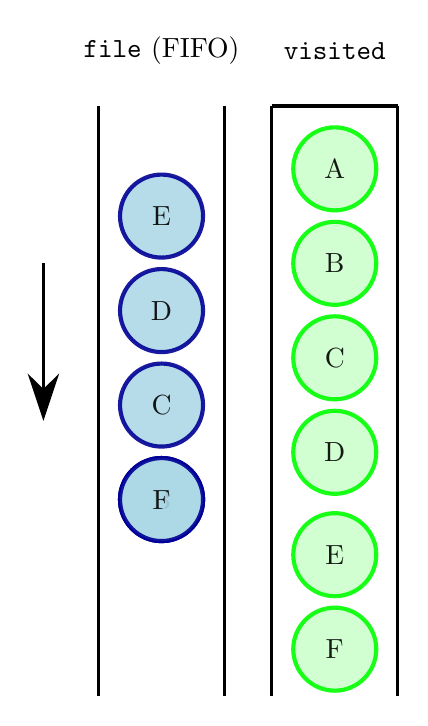
\begin{tikzpicture}[
    filebox/.style={
        draw,
        very thick
    },
    item/.style={
        circle,
        draw=DarkBlueContour,
        fill=LightBlueFill,
        minimum size=30pt,
        inner sep=0pt,
        line width=1.5pt,
        fill opacity=0.9,
        draw opacity = 0.9
    }
]

\draw (-0.4,3.7) node {\texttt{file} (FIFO)};
\draw (1.8,3.7) node {\texttt{visited}};

% file container
% Left and right walls (no lids)
\draw[filebox] (-1.2, 3) -- (-1.2, -4.5);
\draw[filebox] ( 0.4, 3) -- ( 0.4, -4.5);

% visited list
\draw[filebox] (1, 3) -- (1, -4.5);
\draw[filebox] (2.6, 3) -- ( 2.6, -4.5);
\draw[filebox] (1, 3) -- ( 2.6, 3); % top lid

% \draw[-{Stealth[length=3mm, width=3mm]}, thick] (-0.5,-3) arc [start angle=-180, end angle=0, radius=1.15];


% Items stacked vertically
\onslide<1>{\node[item] (A) at (-0.4, -2) {A};}
\onslide<3-6>{\node[item] (B) at (-0.4, -2) {B};}
\onslide<4-7>{\node[item] (C) at (-0.4, -0.8) {C};}
\onslide<5-8>{\node[item] (D) at (-0.4, 0.4) {D};}
\onslide<6-10>{\node[item] (E) at (-0.4, 1.6) {E};}
\onslide<12>{\node[item] (F) at (-0.4, -2) {F};}

% visited
\onslide<1->{\node[item, fill=green!20, draw=green] (A) at (1.8, 2.2) {A};}
\onslide<3->{\node[item, fill=green!20, draw=green] (B) at (1.8, 1.0) {B};}
\onslide<4->{\node[item, fill=green!20, draw=green] (C) at (1.8, -0.2) {C};}
\onslide<5->{\node[item, fill=green!20, draw=green] (D) at (1.8, -1.4) {D};}
\onslide<6->{\node[item, fill=green!20, draw=green] (E) at (1.8, -2.7) {E};}
\onslide<12->{\node[item, fill=green!20, draw=green] (F) at (1.8, -3.9) {F};}

% Arrows
\draw[-{Stealth[length=6mm, width=4mm]}, thick]  (-1.9,1) -- (-1.9,-1);

\end{tikzpicture}
}
\end{minipage}
\hfill
\begin{minipage}{0.7\textwidth}
    \begin{center}
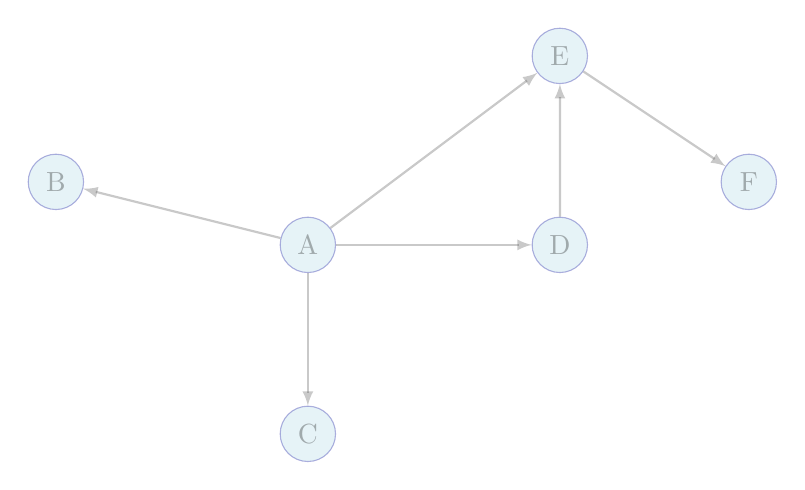
\begin{tikzpicture}[scale=1.6]

% --- Node style (dark blue) --

% --- Nodes (coordinates chosen to match your picture) ---
\node[vertex, highlight=<1->] (A) at (0,0) {A};
\node[vertex, highlight=<3->] (B) at (-2,0.5) {B};
\node[vertex, highlight=<4->] (C) at (0,-1.5) {C};
\node[vertex, highlight=<5->] (D) at (2,0) {D};
\node[vertex, highlight=<6->] (E) at (2,1.5) {E};
\node[vertex, highlight=<12-13>] (F) at (3.5,0.5) {F}; % upper-left node

% --- Edges ---
% \draw[edge, <-] (F) -- (E);
\draw[edge, <-, highlight=<6->] (E) -- (A);
\draw[edge, ->, highlight=<5->] (A) -- (D);
\draw[edge, ->, highlight=<4->] (A) -- (C);
\draw[edge, ->, highlight=<12->] (E) -- (F);

\draw[edge, <-, highlight=<3->] (B) -- (A);
\draw[edge, ->, highlight=<10->] (D) -- (E);

\end{tikzpicture}
\end{center}
\end{minipage}





\begin{itemize}
\item<1-> \texttt{order}: \only<1>{[]}\only<2-6>{[A]}\only<7>{[A, B]}\only<8>{[A, B, C]}\only<9-10>{[A, B, C, D]}\only<11>{[A, B, C, D, E]}\only<12>{[A, B, C, D, E]}\only<13>{[A, B, C, D, E, F]}
\item<2-> \only<2>{Une fois A retiré de la file, on le met dans \texttt{order}.} \only<3>{Et on explore les voisins de A — ici B}
 \only<4>{On explore C} \only<5>{On explore D} \only<6>{On explore E} \only<7>{Une fois tous les voisins de A explorés, on retire de la file B et on le met dans \texttt{order}.} \only<8>{B n'a pas de voisins — on retire C de la file et on le met dans \texttt{order}.} \only<9>{C n'a pas de voisins — on retire D de la file et on le met dans \texttt{order}.} \only<10>{D a le voisin E — mais E est déjà dans visited.}
 \only<11>{On retire E de la file et on le met dans \texttt{order}.} \only<12>{On explore les voisins de E.} \only<13>{On retire F de la file et on le met dans \texttt{order}.}
\end{itemize}
\end{frame}

\end{document}